\documentclass[12pt,a4paper,fontset=none]{ctexart}
\usepackage{amsmath,amssymb,array,booktabs,geometry,graphicx,tabularx,xurl}
\usepackage[numbers,sort&compress]{natbib}
\usepackage{hyperref}
\setCJKmainfont[BoldFont=Noto Serif CJK SC Bold]{Noto Serif CJK SC}
\setCJKsansfont[BoldFont=Noto Sans CJK SC Bold]{Noto Sans CJK SC}
\setCJKmonofont[BoldFont=Noto Sans Mono CJK SC Bold]{Noto Sans Mono CJK SC}
\geometry{margin=2.4cm}
\hypersetup{colorlinks=true,linkcolor=blue,citecolor=blue,urlcolor=blue}
\newcolumntype{Y}{>{\raggedright\arraybackslash}X}
\setlength{\emergencystretch}{3em}
\title{面向可审计实体关系抽取的溯源保持与证据门控知识图谱增强}
\author{匿名作者（中文核对稿）}
\date{}
\begin{document}
\maketitle
\begin{abstract}
将文本转化为结构化知识，不仅需要准确抽取实体与关系，还需要明确连接预测关系
与原文证据。知识图谱能够提供领域上下文，但检索到的关联并不必然是当前句子中
陈述的事实。本文提出一种保持溯源信息的证据门控框架，将图谱引导的候选生成与
结果接受分离。训练集图谱向紧凑式生成抽取器提供有界概念与关系提示，确定性跨度
重建、实体选择和关系验证则共同形成带证据链接的断言图谱。实验在ADE和CoNLL04
上开展，采用统一字符跨度评估协议，分别考察药物不良反应抽取和通用实体关系抽取。
在模型比较之前，通过数据统计刻画标签集中程度、句长以及数据划分组成。已完成
测试表明，所提系统在两个基准上的关系F1均高于配对的纯源生成器，同时提高关系
精确率并保留明确的门控决策记录。研究为受控图谱增强与面向人工复核的原文落地
预测提供了可实现机制，并明确区分结构准入条件与语义正确性。
\end{abstract}
\noindent\textbf{关键词：}实体关系抽取；知识图谱；溯源；证据落地；药物不良反应；选择性预测

\section{引言}
\label{sec:introduction}
结构化信息抽取连接非结构化文本与可检索的实体、类型关系及下游知识系统。
在安全相关应用中，抽取关联还必须可供检查：使用者需要知道识别的是哪一个提及、
哪一句原文支持该关系，以及哪些处理步骤产生了最终断言。药物不良反应抽取直接
体现了这一要求。即使输出结构合法，模型若识别出药物和不良反应后虚构二者之间的
关联，仍会形成误导性记录。通用信息抽取则在更丰富的实体和关系类型上，对同一
技术问题提供补充检验。

神经实体与关系模型已经为识别问题提供了有效方法\cite{li2022ner,eberts2020spert}。
生成式模型允许在不同标签集合间复用统一的结构化输出格式，但流畅生成不保证
预测对象受到输入支持\cite{ji2023hallucination}。当抽取三元组进入知识图谱后，
错误可能被后续检索或推理使用，从而超出原始句子的范围传播。

知识图谱能够提供类型化领域先验\cite{hogan2021kg}，检索增强使模型无需完全依靠
参数记忆即可访问这些先验\cite{lewis2020rag}。与此同时，它引入了事实依据的权威性
问题：训练句中出现过的关系可以提示应寻找什么，却不能证明新句子也具有该关系。
训练图谱还可能返回当前训练样本自身的标注，或暴露跨划分共享内容。因此，研究
问题不仅是图谱是否提高召回率，还包括上下文是否有资格进入提示，以及其作用是否
能够得到控制与审计。

本文采用分阶段架构处理这一问题。纯源、精确锚点和高召回图谱条件生成器分别训练，
形成输入条件的配对比较。确定性关系验证器检查结构与原文证据条件，互补的实体门控
通过生成器一致性、原文匹配锚点或验证关系端点接受部分候选。最终系统将接受实体与
端点存活的验证关系组合。本文使用已有表示和适配技术，贡献在于对这些组件的受控
组合，而不是新骨干模型或新的优化算法。

本文聚焦ADE\cite{gurulingappa2012ade}和CoNLL04\cite{roth2004conll}。
ADE是药物安全相关抽取任务，包含两种实体与一种关系标签；CoNLL04作为通用领域
对照，包含四种实体与五种有向关系标签。二者均使用英文句级输入，使研究可以聚焦
抽取与验证机制，而不混入长文档窗口构造问题。两个数据集分别训练、分别评估，
本实验不是从一个数据集直接迁移到另一个数据集的零样本迁移实验。

主要贡献包括：
\begin{itemize}
\item 提出带溯源约束的图谱上下文策略，仅使用训练标注，排除当前样本独有支持的
候选，并对训练与评估文本完全重合的句子清空图谱提示。
\item 以确定性方式组合原文跨度重建、实体选择和关系验证，保留带证据链接的断言，
记录接受或拒绝预测的原因。
\item 提供可复现的双基准分析，将划分与标签统计、统一严格跨度计分、验证集消融、
已完成测试比较和完全重合文本敏感性分析联系起来。
\end{itemize}
本文面向分析人员使用的知识系统提供可审计抽取层，不将基准关系标签直接解释为
临床因果，不输出经过校准的风险概率，也不据此宣称自主安全决策已经得到验证。

\section{相关工作}
\label{sec:related}
\subsection{联合实体关系抽取}
实体识别必须同时解决提及边界与类型，关系抽取还依赖正确恢复有方向的类型端点
\cite{li2022ner}。在该任务中，全局一致性约束具有较长研究历史，CoNLL04对应的
研究即采用全局推断形式\cite{roth2004conll}。SpERT枚举候选跨度，利用预训练
Transformer联合建模实体与关系\cite{eberts2020spert}。由于其完成相同联合任务而不
依赖生成式JSON接口，它是重要对照。本文从干净基础编码器重新训练SpERT，采用
相同训练划分，不使用可能包含开发集数据的已发布任务检查点。

GLiNER和GLiREL分别提供标签条件实体识别与关系分类方案
\cite{zaratiana2024gliner,boylan2025glirel}。它们与本地微调生成器在监督方式、
预训练和输出构造上不同，因此本文报告具体实现的训练集校准流水线，而不是对整个
模型家族作穷尽性结论。同骨干零样本生成器进一步帮助区分本地适配与图谱条件的作用。

\subsection{图谱上下文与约束生成}
知识图谱显式表示实体与类型关系，检索增强将选中记录作为模型上下文
\cite{hogan2021kg,lewis2020rag}。GenIE通过结构化输出空间和实体、关系目录约束
生成式信息抽取\cite{josifoski2022genie}。但目录合法性和原文支持是不同条件：
一个合法实体或关系仍可能没有在当前输入中被陈述。因此，本文将图谱上下文视为
候选先验，其准入取决于训练溯源与局部原文匹配。

BGE-M3为语义模式检索提供冻结文本表示\cite{chen2024bgem3}，它既不是图神经网络，
也不与抽取器联合优化。QLoRA支持Qwen3骨干的紧凑式适配
\cite{dettmers2023qlora,qwen2025qwen3}。但两者本身均没有定义候选是否应进入最终
断言图谱，本文门控将这一接受策略显式化。

\subsection{证据与安全相关知识构建}
幻觉研究区分了结构良好的输出与忠实于原文的输出\cite{ji2023hallucination}。
事故报告的提示式图谱构建也说明了生成知识需要追踪原始来源
\cite{liu2025llmaccidentkg}。ADE为药物安全相关关系任务提供了更受控的评估环境
\cite{gurulingappa2012ade}。不过，ADE标签是文本关联标注，而不是针对患者的因果
结论。本文评估抽取与已实现证据条件，不评估下游决策的医学或运行有效性。

\section{数据集与分布分析}
\label{sec:data}
\subsection{基准来源与划分}
本文采用以SpERT格式发布的句级ADE和CoNLL04文件，计数对应这一预处理版本，
而非原始来源语料中的全部句子。CoNLL04保留其训练、开发与
测试划分。ADE文件包含3,845个训练句和427个测试句，从原始训练池中确定性划出
384句作为开发集，剩余3,461句用于训练。划分以固定种子字符串
\texttt{public-full-42}和原始记录标识符构造字符串，并按SHA-256摘要排序，
而非依据验证表现选样。这是一个固定ADE划分，不是文献中部分研究所采用的多折均值。

表\ref{tab:data}由实际导入资产重新统计。软件称为文档的评估单元对应一个基准句子，
并非完整病案或新闻文章。两套数据均为英文，因此实验不支持多语言或跨语言结论。
发布标注直接导入，不是本项目重新标注的语料。
\begin{table}[htbp]
\centering\small\setlength{\tabcolsep}{4pt}
\caption{实际实验划分的数据清单。依次列出数据集、划分、句数、实体数、关系数与
平均长度；长度为重建原文中的空白分隔词元数。}
\label{tab:data}
\begin{tabular}{llrrrr}
\toprule
Dataset & Split & Sentences & Entities & Relations & Mean length \\
\midrule
ADE & train & 3461 & 8717 & 5470 & 21.17 \\
ADE & validation & 384 & 996 & 627 & 21.82 \\
ADE & test & 427 & 1126 & 724 & 21.24 \\
CoNLL04 & train & 922 & 3377 & 1283 & 28.77 \\
CoNLL04 & validation & 231 & 893 & 343 & 30.27 \\
CoNLL04 & test & 288 & 1079 & 422 & 28.94 \\
\bottomrule
\end{tabular}

\end{table}

\subsection{实体与关系标签分布}
ADE包含\texttt{Drug}、\texttt{Adverse-Effect}两种实体，以及
\texttt{Adverse-Effect}一种关系。导入文件的端点方向是“不良反应指向药物”，
本文保留该约定，不将其改成直觉上的“药物指向不良反应”。CoNLL04的实体类型为
\texttt{Loc}、\texttt{Org}、\texttt{Peop}与\texttt{Other}，关系类型为
\texttt{Work\_For}、\texttt{Kill}、\texttt{OrgBased\_In}、\texttt{Live\_In}
和\texttt{Located\_In}。

图\ref{fig:labels}展示训练标签分布，附录\ref{app:labels}列出每个划分的精确标签
计数。ADE仅有一种关系类型，减少了关系类别之间的混淆，但端点识别、方向和错误
实体配对仍需解决。CoNLL04的关系集合与实体角色更加多样。因此，ADE取得较高
总体F1不意味着药物安全推理天然比通用推理容易，二者的监督抽取任务规模与结构不同。
\begin{figure}[htbp]
\centering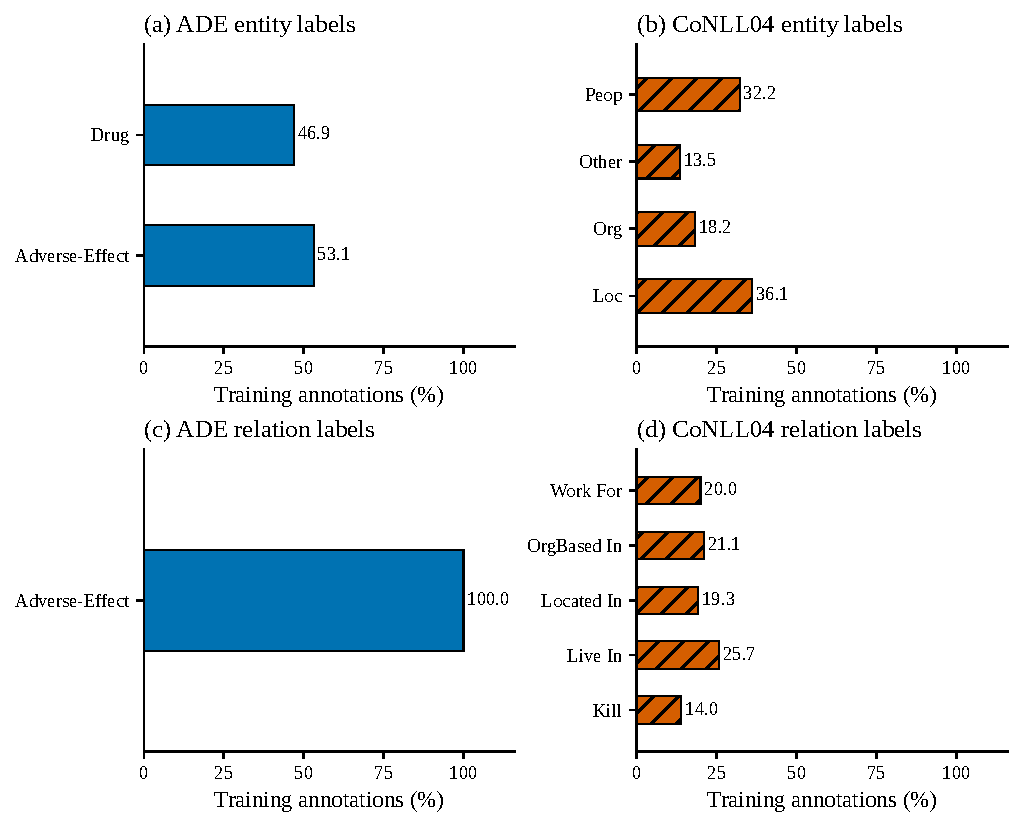
\includegraphics[width=\textwidth]{../figures/ade_conll04/01-label-distribution.pdf}
\caption{训练标注分布。每个子图分别以对应实体或关系总数为分母，不将两种对象
混合计数。颜色与填充纹理同时用于区分两个基准。}
\label{fig:labels}
\end{figure}

\subsection{句长与覆盖范围}
ADE和CoNLL04的平均训练长度分别为21.17与28.77个重建词元，平均测试长度为
21.24与28.94。图\ref{fig:lengths}的累计分布展示全部三个划分，而非仅训练集。
这些是描述性空白分隔词元数，不是Qwen分词器计数。跨导入划分的最大长度分别为
ADE的97与CoNLL04的118。

每个导入句子均至少有一条标注关系。这是所选基准文件的重要特点：它们不衡量
以大量无关句为主的部署文本流上的误报表现。本文保留给定基准组成，没有为所报告
测试额外构造无关系负例句。
\begin{figure}[htbp]
\centering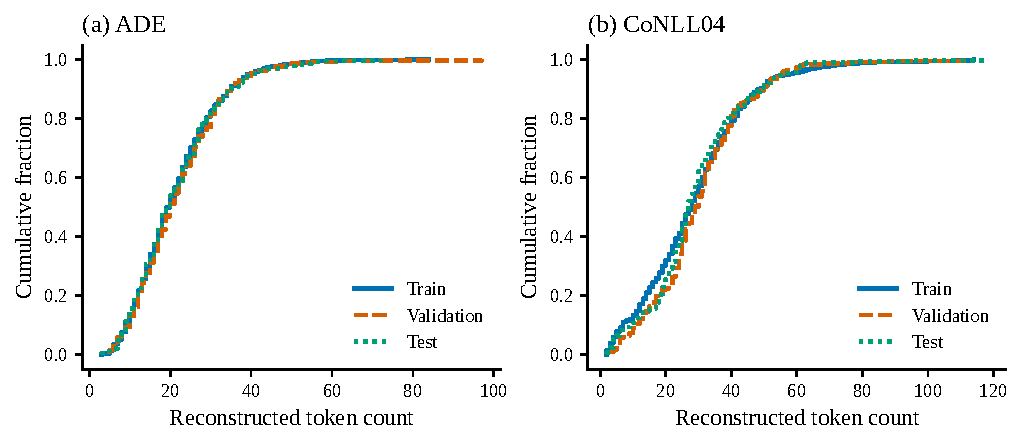
\includegraphics[width=\textwidth]{../figures/ade_conll04/02-sentence-length-distribution.pdf}
\caption{各划分的经验累计句长分布。长度来自确定性重建文本，句级输入未采用
标注辅助的窗口选择。}
\label{fig:lengths}
\end{figure}

\subsection{划分重合与图谱上下文隔离}
两个数据集分别使用各自训练标注构图。完全重合检查先对原文进行大小写折叠与
空白压缩，再比较字符串。ADE未发现训练—开发或训练—测试完全重合；CoNLL04有
14个开发句和19个测试句与训练文本相同。对这些句子，在生成前同时清空精确锚点和
高召回图谱上下文。

清空图谱提示不能撤销生成器对重复训练文本的学习。因此，主比较保留发布划分，
另外使用固定预测，排除19个重合CoNLL04测试句进行敏感性分析。本文不宣称该基准
具有重复簇隔离，也不宣称完全匹配能发现全部近重复内容。

\section{所提方法}
\label{sec:method}
\subsection{原文落地表示}
设句子$x$由发布词元使用单个空格确定性连接。实体提及表示为
\begin{equation}
e=(b,u,y),\qquad x[b:u]=m,
\label{eq:entity}
\end{equation}
其中$[b,u)$为字符区间，$y$为实体标签，$m$为复制的提及文本。关系$r=(e_s,z,e_t)$
包含有向、带类型的端点与关系标签$z$，对象另存来源标识与证据跨度。相同字符串
位于不同偏移时仍是不同提及。公式\eqref{eq:entity}防止仅凭规范化名称便将错误
出现位置计为正确。

导入基准为每条关系赋予\texttt{explicit}状态，以其来源句作为证据跨度。这是
表示约定，不是新增的最小因果证据或不确定性标注。由于端点处于同一句输入，
证据共现在本实验中是相对较弱的条件。

\subsection{架构与比较系统}
图\ref{fig:architecture}展示流水线。SOE（纯源抽取）、EAE（精确锚点抽取）和
HRGE（高召回图谱抽取）在相同Qwen3-4B快照上分别训练QLoRA适配器。SOE使用
原文与训练推导本体，不接收图谱提示；EAE接收保守概念提示；HRGE接收有界锚点、
边先验和语义关系模式。

EVGE（证据验证图谱抽取）对HRGE应用关系验证器。CFE（保守融合抽取）将接受的
HRGE实体与端点过滤后的原始HRGE关系组合。PGE（溯源门控抽取）则将相同实体集合
与端点过滤后的验证关系组合。这三者是确定性后处理变体，而非额外训练网络。
部署PGE需要EAE与HRGE候选，SOE只作为比较分支，不参与融合。
\begin{figure}[htbp]
\centering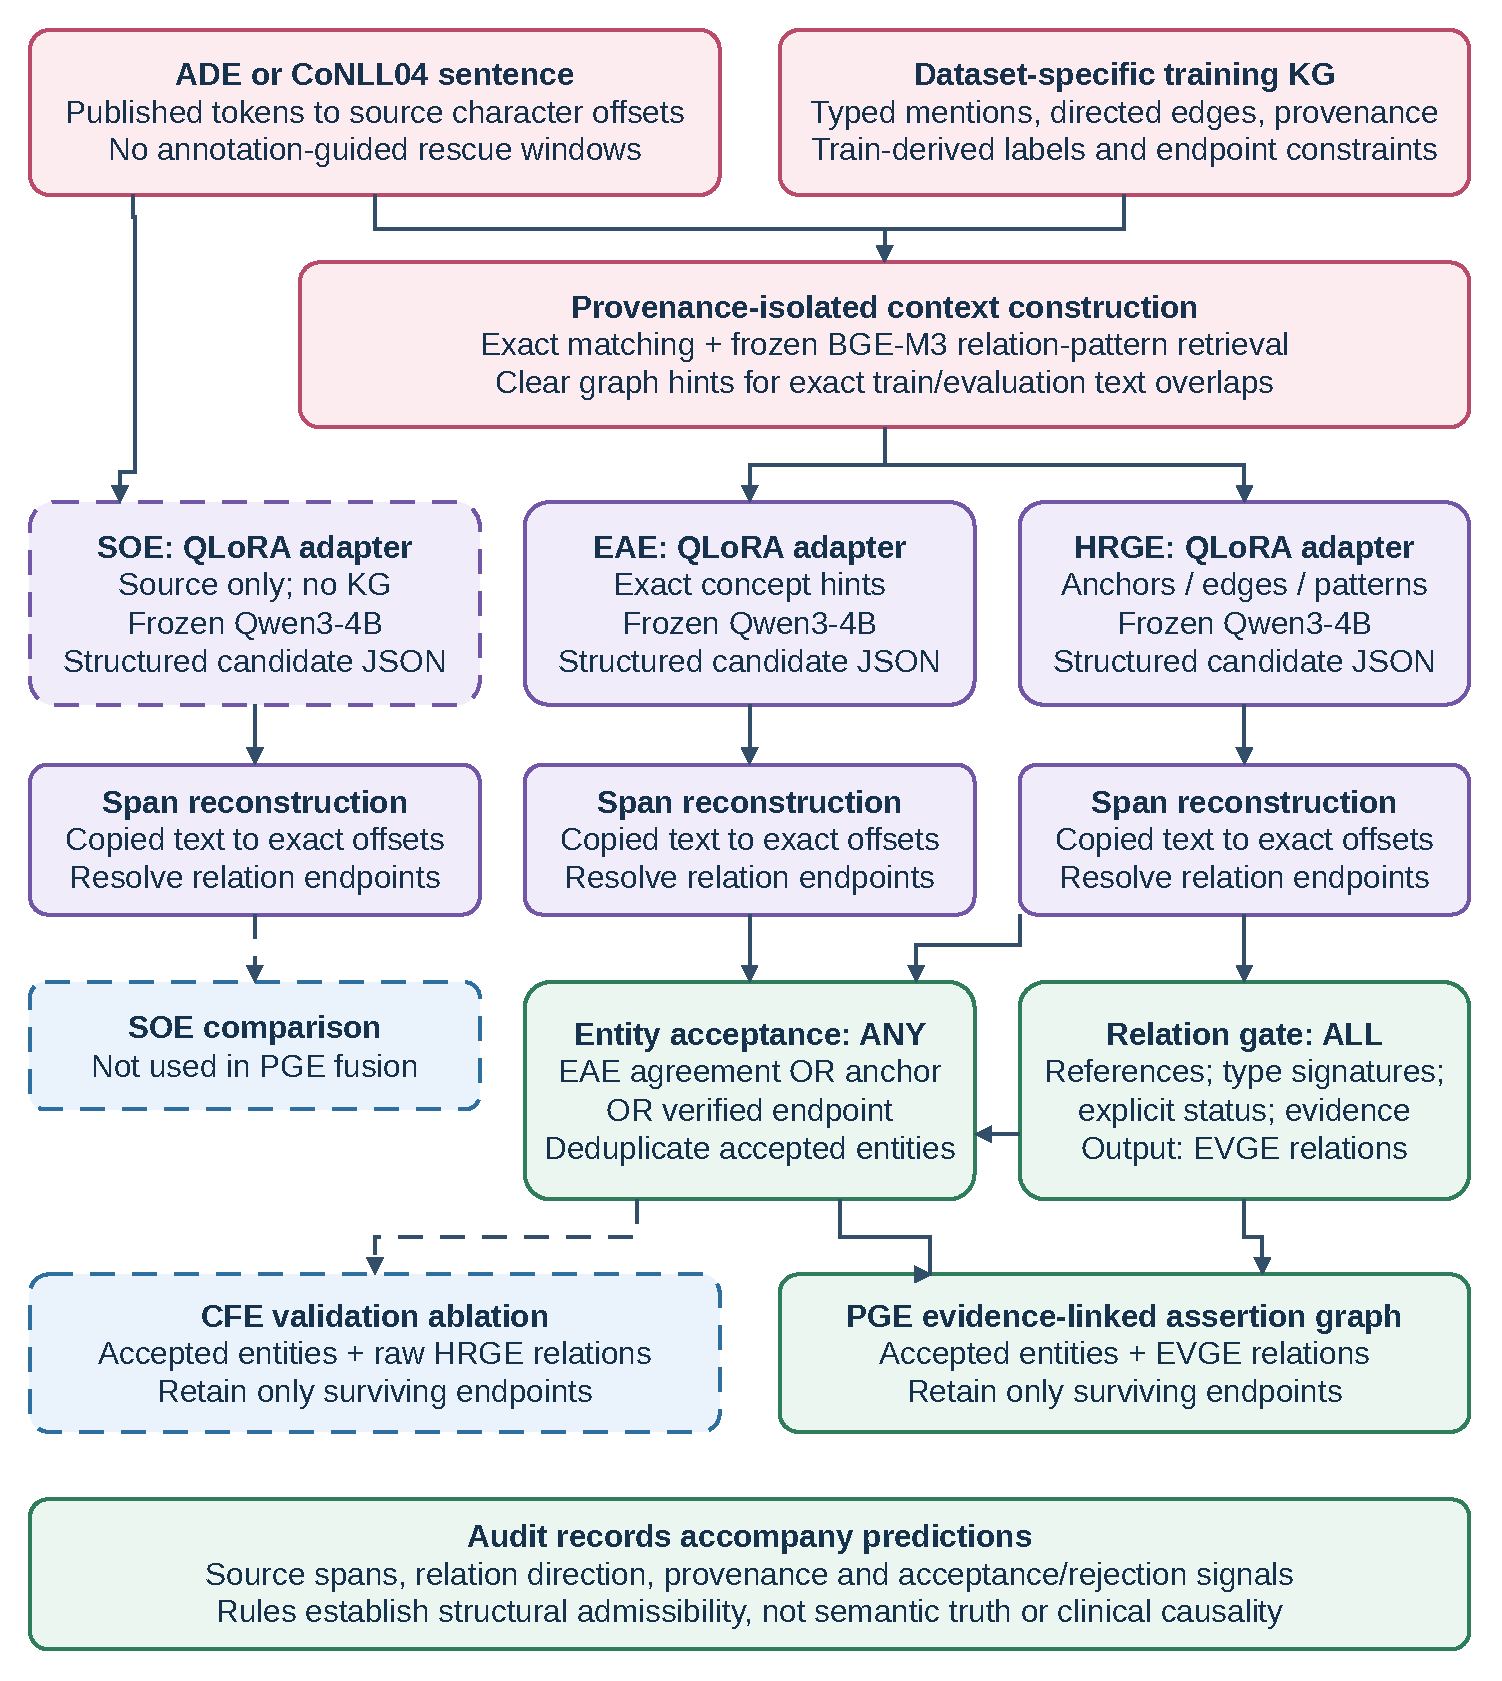
\includegraphics[width=\textwidth]{../figures/ade_conll04/03-pge-architecture.pdf}
\caption{双基准实验架构。各数据集训练图谱提供候选上下文，当前句子提供证据。
三个独立适配器采用相同骨干配置。实体接受要求任一信号成立，关系验证要求全部
检查通过；PGE只保留端点存活的验证关系。虚线框表示比较路径，门控不是学习式网络。}
\label{fig:architecture}
\end{figure}

\subsection{溯源受控图谱上下文}
训练图谱存储提及字符串、类型、有向关系和支持句标识。对训练句$d$，如果候选
只有$d$这一支持来源，则将其排除。存在其他支持句的候选仍有资格保留，其聚合
支持统计不会按完整留一法重新构图。因此，该策略不应被解释为完全删除当前样本
对所有统计量的贡献。

EAE最多使用20个类型平衡的精确概念提示。HRGE具有三个上下文通道：第一，
原文匹配锚点须满足0.8的经验类型纯度及至少4字符的英文长度条件；第二，类型边
先验须在当前样本之外得到支持，且两个端点字符串都在当前原文中出现；第三，
冻结BGE-M3检索语义相关的关系模式记录。设$\mathbf H$存储合格记录的归一化向量，
$\mathbf q$为归一化原文向量，则
\begin{equation}
\mathbf{s}=\mathbf{H}\mathbf{q},\qquad
\mathcal I=\operatorname{TopK}_{k}\{i:s_i\geq\tau\}.
\label{eq:retrieval}
\end{equation}
公式\eqref{eq:retrieval}排序的是候选上下文而非被接受的事实。冻结HRGE上限为
12个锚点（每类最多2个）、6个边先验及4个余弦相似度不低于0.72的语义模式。
提示明确将这些对象称为候选提示；完全重合隔离规则优先于检索，对受影响的评估句
清空全部图谱上下文。

\subsection{紧凑生成与确定性重建}
生成器输出实体标识、复制文本与类型，以及关系标识、有向端点引用、类型和显式
状态，不要求模型计算原文偏移。确定性扩展将复制提及分配到句中出现位置并重建
字符跨度，同时记录无法匹配的字符串与无效引用。这将候选生成与原文坐标处理分离。

三个生成器均训练1轮，批大小1，梯度累积4，学习率$2\times10^{-4}$。
QLoRA使用秩8、alpha 16、dropout 0.05、NF4双重量化与bfloat16计算，适配注意力
q/k/v/o及前馈gate/up/down投影，冻结骨干。AdamW其余参数采用PyTorch默认值，
无学习率调度器或预热。最大训练序列为4,096 token，损失不包含提示token。
所有分支使用相同数据集划分，主比较的训练种子均为42。

推理采用记录中的4,096-token输入上限、1,024-token生成预算和90秒任务时限，
在本地GPU上运行两个推理工作进程。骨干版本与输入哈希保存在产物清单中。失败
任务视为空预测，而非从分母删除。实验使用完整给定句子，不采用标注指导的救援
窗口或依赖标签的句子截断。

\subsection{关系验证与实体接受}
对关系类型$z$，训练标注推导允许的源类型集$S_z$与目标类型集$T_z$。实现检查
$y_s\in S_z$、$y_t\in T_z$，不额外要求每个具体源目标类型组合曾共同出现。
验证器$V(r)$还检查端点引用存在且不同、关系类型已知、状态为显式、证据合法，
以及两个端点字符串都出现在同一局部证据跨度中。接受关系集为
\begin{equation}
R_V=\{r\in R_H:V(r)=1\}.
\label{eq:verifier}
\end{equation}
实体门控使用三个布尔信号：
\begin{equation}
A(e)=A_{\rm agree}(e)\lor A_{\rm anchor}(e)\lor A_{\rm endpoint}(e),
\quad E_A=\{e\in E_H:A(e)=1\}.
\label{eq:accept}
\end{equation}
一致性指EAE预测出大小写折叠、空白规范化后相同文本与类型；锚点支持要求同类型
且经原文门控的HRGE锚点；端点支持表示该实体参与公式\eqref{eq:verifier}保留的关系。
公式\eqref{eq:accept}中的信号互补，但不是统计独立的证据，验证端点更不是第二位
人工复核者的判断。句内规范化文本与类型重复的候选会被折叠。

令$F(R,E)$仅保留两个引用端点均在$E$中存活的关系，则
\begin{equation}
G_{\rm CFE}=(E_A,F(R_H,E_A)),\qquad
G_{\rm PGE}=(E_A,F(R_V,E_A)).
\label{eq:composition}
\end{equation}
公式\eqref{eq:composition}明确了原始关系融合与验证关系融合的区别。所有接受与
拒绝决定均有记录。保留关系满足已声明规则，但规则本身不能证明句子真正陈述了
模型提出的含义。

\section{实验协议}
\label{sec:experiment}
\subsection{研究问题与范围}
本文考察PGE是否相对SOE改善严格实体、关系抽取；图谱上下文与确定性选择如何
在开发集上发挥作用；以及移除完全重合句后优势是否保留。外部基线用于判断生成式
设计与其他抽取模型家族相比的表现，而不是将超过SOE等同于达到最先进水平。

本文的双基准报告范围是在查看验证及已有测试结果之后事后收敛的，属于聚焦分析，
并非对全部尝试领域的预注册代表性抽样。在已有协议中，模型与门控设置在测试开放
之前冻结；SOE和PGE在验证
关系F1退化不超过1个百分点、完成性与证据检查通过后晋级。这是实用的点估计门槛，
而不是统计非劣效检验。本文使用已完成的seed 42测试，不据此推断多种子稳定性。

\subsection{基线与评估一致性}
内部开发集比较包含六个命名系统。测试表包含两个晋级系统及三个已完成外部对照。
Qwen3-4B零样本使用同骨干但不加载本地适配器，并采用已记录的原文扩展和关系验证器。
SpERT从\texttt{bert-base-cased}出发，在相同训练划分上训练20轮，批大小2，关系
阈值0.4；使用最终检查点，不挑选测试最优轮次。GLiNER+GLiREL使用预测实体而非
金标实体，关系校准局限于训练集内部子集，实体阈值为0.5。这些配置不同，不构成
等计算量比较。

记录中的GLiREL校准为ADE选择原始规范标签与0.0关系阈值，为CoNLL04选择自然
语言化标签与0.1关系阈值。选择这些设置没有使用开发或测试金标。

主表全部预测使用同一个公开数据字符跨度评估器重新计分。实体键包含精确原文
区间和类型，关系键包含两个带类型的有向端点键及关系标签。预测证据偏移必须
在给定原文中有效，评估器不通过搜索规范化文本来补救缺失偏移。重复键只计一次，
无效对象保留为未匹配预测，缺失任务视为空输出。对合并计数，定义
\begin{equation}
P=\frac{TP}{TP+FP},\quad R=\frac{TP}{TP+FN},\quad
F_1=\frac{2TP}{2TP+FP+FN}.
\label{eq:metrics}
\end{equation}
公式\eqref{eq:metrics}在各数据集内跨句合并使用，不对单句F1再求平均。
所有导入状态均为显式，因此带状态分数不构成独立的不确定性评估。
统一评估器消除了旧重复处理方式导致的小幅分母差异，原始资产不变，另提供新旧
计数对照报告。

\subsection{统计与规则符合性分析}
本文固定预测，以种子20260830对测试句进行20,000次配对bootstrap，每次重新
计算合并F1。百分位区间描述该已完成模型对的句子抽样不确定性，不描述训练种子
差异。区间为描述性结果，未进行多重比较校正，也不用于改变冻结模型或门控。

证据覆盖率与规则无效计数独立于抽取F1报告，采用评估器去重之前的预测对象作为
分母。完全重合敏感性分析从两个系统中移除同一批测试句标识，不重新训练或生成。
本次修订读取测试标签仅用于统计与计分，不用于图谱提示构造或阈值选择。

\section{结果}
\label{sec:results}
\subsection{已完成测试比较}
表\ref{tab:test}给出统一评估器下的测试结果。ADE上，PGE将关系精确率从80.62\%
提高到87.00\%，召回率从67.82\%提高到72.10\%，关系F1由SOE的73.67\%提高到
78.85\%。实体F1基本不变，分别为87.97\%与87.93\%。因此，主要改善发生在关系
抽取，而不是普遍改善实体提及识别。

CoNLL04上，关系精确率由54.61\%提高到62.40\%，召回率由56.16\%提高到57.82\%，
关系F1由55.37\%提高到60.02\%；实体F1则由83.83\%降至83.20\%。该次运行以部分
实体覆盖为代价，获得了更好的关系精确率与召回率平衡。
\begin{table}[htbp]
\centering\scriptsize\setlength{\tabcolsep}{2.6pt}
\caption{已完成测试比较，严格原文字符跨度微平均分数（\%）。Qwen3-ZS为
Qwen3-4B零样本加已记录验证器；GLiNER+GLiREL仅在训练数据内校准。各数据集使用
自身测试划分，本地训练系统采用seed 42，所有行采用同一评估器重算。}
\label{tab:test}
\begin{tabular}{llrrrrrr}
\toprule
Dataset & System & Ent. P & Ent. R & Ent. F1 & Rel. P & Rel. R & Rel. F1 \\
\midrule
ADE & Qwen3-ZS + verifier & 63.83 & 63.32 & 63.58 & 39.36 & 22.24 & 28.42 \\
ADE & GLiNER + GLiREL & 79.30 & 64.65 & 71.23 & 60.31 & 43.23 & 50.36 \\
ADE & SOE & 92.21 & $\mathbf{84.10}\uparrow$ & $\mathbf{87.97}\uparrow$ & 80.62 & 67.82 & 73.67 \\
ADE & PGE & $\mathbf{92.89}\uparrow$ & 83.48 & 87.93 & $\mathbf{87.00}\uparrow$ & $\mathbf{72.10}\uparrow$ & $\mathbf{78.85}\uparrow$ \\
CoNLL04 & Qwen3-ZS + verifier & 48.78 & 53.94 & 51.23 & 30.92 & 19.19 & 23.68 \\
CoNLL04 & GLiNER + GLiREL & 60.78 & 14.37 & 23.24 & 13.79 & 3.79 & 5.95 \\
CoNLL04 & SOE & 85.83 & $\mathbf{81.93}\uparrow$ & $\mathbf{83.83}\uparrow$ & 54.61 & 56.16 & 55.37 \\
CoNLL04 & PGE & $\mathbf{86.04}\uparrow$ & 80.54 & 83.20 & $\mathbf{62.40}\uparrow$ & $\mathbf{57.82}\uparrow$ & $\mathbf{60.02}\uparrow$ \\
\bottomrule
\end{tabular}

\end{table}

SpERT在已完成系统中取得最高实体与关系F1：ADE为91.37\%／84.08\%，CoNLL04为
89.02\%／69.72\%。PGE改善了配对生成式基线，但没有超过该训练式跨度模型。
同时，PGE在两套数据的两类任务上均超过记录中的零样本与GLiNER+GLiREL流水线；
后者结论仅适用于已实现标签映射和校准设置，并不意味着这些家族的所有配置均较差。

\subsection{配对差异与不确定性}
从未四舍五入计数计算，ADE的PGE减SOE关系F1差异为5.18个百分点，配对95\%
区间为[0.31,10.29]；CoNLL04为4.65个百分点，区间[0.04,9.12]。正点估计与主表
改善一致，但区间较宽、下界接近零，应理解为对当前已完成测试预测的证据，而不是
跨种子的普遍保证。实体F1差异为ADE的$-0.04$个百分点，区间[$-1.75$,1.62]；
CoNLL04的$-0.63$个百分点，区间[$-2.38$,1.04]，均不支持实体F1提高的结论。

\subsection{开发集组件分析}
表\ref{tab:ablation}区分开发集上的候选生成与确定性选择。ADE的HRGE关系F1为
76.29\%，超过SOE的73.16\%；EVGE与HRGE相同，PGE与CFE相同，说明关系验证器
在这些变体中没有进一步删去关系。实体门控降低HRGE召回率，最终PGE关系F1为
75.91\%。因此，不能将ADE全部增益归因于验证，也不能宣称每个阶段都独立提高F1。

CoNLL04上，HRGE关系F1为58.26\%，低于SOE的60.24\%；验证提高到59.60\%，最终
组合达到60.19\%。在开发集点估计上，这与SOE基本持平，而不是明显增益。门控后
实体精确率提高，召回率与F1降低。本文保留开发与测试表现的差异，不以测试结果
重新选择消融系统。
\begin{table}[htbp]
\centering\scriptsize\setlength{\tabcolsep}{3pt}
\caption{统一严格跨度评估器下的开发集消融（微平均\%，seed 42）。这些行用于
分析冻结架构，不代表额外晋级的测试系统。}
\label{tab:ablation}
\begin{tabular}{llrrrrrr}
\toprule
Dataset & System & Ent. P & Ent. R & Ent. F1 & Rel. P & Rel. R & Rel. F1 \\
\midrule
ADE & SOE & 89.25 & 82.53 & 85.76 & 78.82 & 68.26 & 73.16 \\
ADE & EAE & 90.49 & 81.22 & 85.61 & 80.84 & 67.30 & 73.46 \\
ADE & HRGE & 90.35 & 85.54 & 87.88 & 80.04 & 72.89 & 76.29 \\
ADE & EVGE & 90.35 & 85.54 & 87.88 & 80.04 & 72.89 & 76.29 \\
ADE & CFE & 90.48 & 83.94 & 87.08 & 81.39 & 71.13 & 75.91 \\
ADE & PGE & 90.48 & 83.94 & 87.08 & 81.39 & 71.13 & 75.91 \\
CoNLL04 & SOE & 84.94 & 82.08 & 83.49 & 61.33 & 59.18 & 60.24 \\
CoNLL04 & EAE & 83.71 & 82.87 & 83.29 & 58.10 & 60.64 & 59.34 \\
CoNLL04 & HRGE & 82.35 & 81.52 & 81.94 & 60.06 & 56.56 & 58.26 \\
CoNLL04 & EVGE & 82.35 & 81.52 & 81.94 & 62.99 & 56.56 & 59.60 \\
CoNLL04 & CFE & 84.97 & 78.50 & 81.61 & 63.37 & 55.98 & 59.44 \\
CoNLL04 & PGE & 84.97 & 78.50 & 81.61 & 65.08 & 55.98 & 60.19 \\
\bottomrule
\end{tabular}

\end{table}

\subsection{规则符合性及其解释}
测试SOE在ADE的610个关系对象中包含31个规则无效对象，在CoNLL04的436个关系
对象中包含16个。PGE分别保留600与392个关系对象，规则无效对象均为零。HRGE的
ADE无效关系已经为零；CoNLL04的413个对象中只有3个无效关系。这些计数区分了
候选本身质量与验证器的贡献。

两个测试集上，SOE、HRGE、PGE测得的无支持证据计数均为零。由于证据是完整句子，
端点成功绑定之后容易满足共现。因此，本实验没有证明将非零无支持率降低的效果，
而是展示显式证据绑定与规则符合。基于金标的F1衡量另一性质：类型关系是否与
标注一致。

\subsection{完全重合敏感性分析}
移除19个训练—测试完全重合句后，CoNLL04剩余269个测试句、1,023个金标实体和
403条金标关系。SOE关系F1为53.79\%，PGE为59.10\%，差异5.31个百分点；实体F1
分别为83.02\%与82.90\%。关系优势在排除这些重合句后仍保留。该分析处理的是
完全重复文本，不覆盖所有语义重合或预训练污染。ADE没有此类重合，敏感性结果
与完整测试一致。

\section{讨论}
\label{sec:discussion}
\subsection{两个基准能够支持什么结论}
共同结果是关系F1相对纯源生成有所提高，而不是普遍优于其他抽取架构。两个测试
均伴随关系精确率提高，实体F1则相近或略降，这与控制候选接受、而非最大化输出量
的设计相符。验证消融进一步说明图谱条件与选择会相互作用：召回导向上下文可在
ADE中发挥作用，却不自动改善CoNLL04；候选已满足规则时，验证器可能不执行额外
过滤。

分布分析有助于解释数据集差异。ADE训练池更大、平均句子更短、关系类型只有一种；
CoNLL04训练句更少、输入更长、关系标签有五种。这些因素同时变化，并未被实验
独立隔离。它们与分数的关联支持分别报告数据集，但不能证明性能差距的因果来源。

\subsection{可审计性是独立设计目标}
系统可能在准确率上不及SpERT，但仍为生成图谱对象提供可检查的接受机制。
其价值在于完整路径可见：图谱支持说明为何建议候选，重建偏移说明出现位置，
门控记录说明接受或拒绝原因。不过，该价值属于架构属性。当前实验没有用户研究
来测量分析人员工作量减少、决策改善或信任提高，不能用完全规则符合替代这些证据。

门控还具有覆盖代价。一致性按规范化文本与类型判断，融合可能折叠重复提及，而
评估器区分其偏移，因而可能丢失合法出现位置。合法端点类型和句内共现不足以证明
关系含义，三个门控信号也不是三次独立确认。因此，最终输出仍是供复核的候选
断言图谱。

\subsection{对安全相关应用的启示}
ADE将实验连接到药物安全信息抽取，CoNLL04则检验通用关系结构。框架可向分析
人员同时呈现候选关系、来源句、类型端点及接受路径的溯源，再由分析人员接受、
修订或拒绝。没有进入保留图谱，不能证明不良反应或其他现实关系不存在。

本任务止步于药物警戒判断、患者级因果归因或实际行动之前。两套数据均未验证
风险传播、韧性评估或自主干预。扩展到这些应用，需要除抽取F1之外的任务结果
指标与专家评估。

\section{局限性与负责任使用}
\label{sec:limitations}
聚焦且事后收敛的报告范围与单个完成训练种子限制了泛化。固定ADE划分不能直接
等同于已发表多折结果。两套数据均为英文含关系句，多语言表现、长报告处理和
无限制文本流上的误报率不在本实验范围内。若缺少上游文章标识，句级bootstrap
不能恢复来自同一原始文章的句间依赖。

完全重合隔离防止为已知重复文本提供直接图谱提示，却没有消除训练暴露；敏感性
分析只排除了已知完全重复。冻结预训练模型也可能接触过相关材料，当前产物不能
排除这一点。本体的允许源类型集与目标类型集，弱于只允许真实观测联合类型对的
约束。

1轮生成器、20轮SpERT与预训练标签条件模型不是等计算量基准。PGE需要两套
适配生成器和冻结检索，不能把紧凑适配等同于经过测量的端到端成本节省。本文没有
新增临床标注或独立证据判断标签。数据与模型公开可得，也不意味着允许所有再分发
或商业使用，原始许可证仍须遵守。

\section{结论}
\label{sec:conclusion}
本文提出溯源保持与证据门控图谱增强框架，在ADE和CoNLL04上评估。数据统计
揭示了两个基准的标签与输入长度差异。统一严格跨度评估下，PGE已完成测试的关系
F1相对SOE分别提高5.18与4.65个百分点，同时提供明确的原文链接接受路径。
CoNLL04关系优势在移除训练—测试完全重合句后仍存在。SpERT在总体抽取F1上仍
更强，开发集消融也说明门控并非在孤立使用时始终有益。所支持的成果是面向人工
复核的受控、可审计图谱增强抽取，而不是普遍准确率领先或自主安全推理已经验证。

\section*{致谢与资助}
作者识别性资助与致谢信息随独立作者页提供，双盲正文中隐藏。
\section*{竞争利益声明}
作者声明不存在可能影响本文工作的已知竞争性经济利益或个人关系。
\section*{数据与代码可用性}
实验使用SpERT格式的公开ADE与CoNLL04数据。匿名复现材料将包含划分构造、
数据统计、来源哈希、评估代码和派生结果表。数据正文与模型权重仍受原始许可证
约束，识别性仓库链接在双盲阶段隐藏。
\section*{生成式人工智能与人工智能辅助技术使用声明}
作者使用OpenAI Codex辅助代码检查、语言编辑、图表制作与论文组织。作者负责
复核相关材料并对最终内容负责；作为研究系统评估的语言模型在方法中另行说明。

\appendix
\section{各划分标签计数}
\label{app:labels}
表\ref{tab:labels}列出分布分析所依据的精确计数。ADE中名称相同的实体标签与
关系标签属于不同标注集合，不能合并。
\begin{table}[htbp]
\centering\small\setlength{\tabcolsep}{4pt}
\caption{导入文件的精确实体与关系计数，分别列出训练、验证和测试划分。}
\label{tab:labels}
\begin{tabular}{lllrrr}
\toprule
Dataset & Kind & Label & Train & Validation & Test \\
\midrule
ADE & Entity & ADVERSE EFFECT & 4631 & 529 & 616 \\
ADE & Entity & DRUG & 4086 & 467 & 510 \\
ADE & Relation & ADVERSE EFFECT & 5470 & 627 & 724 \\
CoNLL04 & Entity & LOCATION & 1219 & 322 & 427 \\
CoNLL04 & Entity & ORGANIZATION & 616 & 170 & 198 \\
CoNLL04 & Entity & OTHER & 455 & 118 & 133 \\
CoNLL04 & Entity & PERSON & 1087 & 283 & 321 \\
CoNLL04 & Relation & KILL & 179 & 42 & 47 \\
CoNLL04 & Relation & LIVE IN & 330 & 91 & 100 \\
CoNLL04 & Relation & LOCATED IN & 247 & 65 & 94 \\
CoNLL04 & Relation & ORGANIZATION BASED IN & 271 & 76 & 105 \\
CoNLL04 & Relation & WORK FOR & 256 & 69 & 76 \\
\bottomrule
\end{tabular}

\end{table}
\begingroup\small
\bibliographystyle{elsarticle-num}
\bibliography{references}
\endgroup
\end{document}
